% This is the file where my Master Thesis will be written. It uses the adapted
% LNCS Template.
%
% I'll be using a few codes in the comments, which can be easily looked up:
% * NOTE: theseis-text related comments
% * TODO: thesis-related TODO's
% * WARN: latex/formatting-related warningss
%
% WARN: for running head, subsititute the line below by:
% \documentclass[runningheads,a4paper]{llncs}
\documentclass{llncs}
%
%%% WARN: custom extension
\usepackage{xcolor}
\newcommand{\todo}[1]{\textcolor{red}{TODO: #1}\PackageWarning{TODO:}{#1!}}

%%% GLOSSARIES
\usepackage{glossaries}

%%% inline code
\usepackage{xparse}
\NewDocumentCommand{\codeword}{v}{%
\texttt{\textcolor{blue}{#1}}%
}

%%% figures
\usepackage{graphicx}
\usepackage{wrapfig}

\makeglossaries

\newacronym{tls}{TLS}{Transport Layer Security}%
\newacronym{ssl}{SSL}{Secure Sockets Layer}%
\newacronym{ietf}{IETF}{Internet Engineering Task Force}%
\newacronym{mac}{MAC}{Message Authentication Code}%
\newacronym{psk}{PSK}{Pre-Shared Key}%
\newacronym{aead}{AEAD}{Authenticated Encryption With Associated Data}%
\newacronym{pkc}{PKC}{Public Key Cryptography}%
\newacronym{hkdf}{hkdf}{HMAC-based Extract-and-Expand Key Derivation Function}%



%%% WARN: added as specified here:
% https://tex.stackexchange.com/questions/272200/table-of-contents-showing-the-title-as-only-entry-latex
\setcounter{tocdepth}{2}
\makeatletter
\renewcommand*\l@author[2]{} % removes author name from TOC
\renewcommand*\l@title[2]{} % removes title name from TOC
\makeatletter
%%%
%
\usepackage{makeidx}  % allows for indexgeneration
%
\begin{document}
%
\frontmatter          % for the preliminaries
%
\pagestyle{headings}  % switches on printing of running heads
%
\addtocmark{TLS For IoT} % additional mark in the TOC

\tableofcontents
\newpage

\mainmatter              % start of the contributions
%
\title{Transport Layer Security Protocol For Internet Of Things}
%
\titlerunning{TLS For IoT}  % abbreviated title (for running head)
%                                     also used for the TOC unless
%                                     \toctitle is used
%
\author{{Illya Gerasymchuk} \\
\email{illya.gerasymchuk@tecnico.uliboa.pt},\\ WWW home page:
\texttt{https://iluxonchik.github.io/}}
%
\authorrunning{Illya Gerasymchuk} % abbreviated author list (for running head)
%
%%%% list of authors for the TOC (use if author list has to be modified)
\tocauthor{Illya Gerasymchuk}
%
\institute{Instituto Superior Técnico}
% WARN: supper hacked-in
\supervisors{Ricardo Chaves, Aleksandar Ilic}
\maketitle              % typeset the title of the contribution

\begin{abstract}
The abstract should summarize the contents of the paper
using at least 70 and at most 150 words. It will be set in 9-point
font size and be inset 1.0 cm from the right and left margins.
There will be two blank lines before and after the Abstract. \dots
\keywords{TLS, IoT, cryptography, protocol, lightweight cryptography}
\end{abstract}
%
\section{Intoduction}
%
\todo{Intruduce the topic: explain what is IoT; what is TLS; what are the issues with
using RAW TLS with IoT(power, computation, limited resources).}
%
\subsection{Goals}
%
\section{Related Work}
%
\todo{Tell that first I describe the parts of TLS that are common to both and then
specialize for TLS 1.2 and TLS 1.3}
%
\subsection{The TLS Protocol}
TLS stands for Transport Layer Security, it's a \textbf{client-server} protocol
that runs on top a \textbf{connection-oriented and reliable transport protocol},
such as \textbf{TCP}. Its main goal is to provide \textbf{privacy} and \textbf{integrity}
between the two communicating peers. Privacy implies that a third party will not
be able to read the data, while integrity means that a third party will not be
able to alter the data.

In the TCP/IP Protocol Stack, \gls{tls} is placed between the \textbf{Transport}
and \textbf{Application} layers. It's designed to make the application developer's
life easier: all the developer has to do is create a "secure" connection, instead
of a "normal" one.

%%% NOTE: place this in intro? Is this even needed?
%%% NOTE: review, rephrase
%%% NOTE: find better placement
\subsubsection{SSL vs TLS: What's The Difference?}
You will find the names \gls{ssl} and \gls{tls} used interchangeably in the literature,
so I think it's important to distinguish both. \gls{tls} is an evolution of the \gls{ssl} protocol. The protocol changed
its name from \gls{ssl} to \gls{tls} when it was
standardized by the \gls{ietf}.\gls{ssl}
was a proprietary protocol owned by Netscape Communications, and The \gls{ietf}
decided that it was a good idea to standarize it, which resulted in \codeword{RFC 2246} \cite{RFC2246},
specifying \gls{tls} 1.0, which was nothing more than a new version \gls{ssl} 3.0,
very few changes were made.
%
% TODO: add some data supporting the TLS 1.2 usage claim
In this document, I'll be concentrating on \gls{tls} 1.2 and \gls{tls} 1.3 protocols.
The first one is the most recently standardized version of \gls{tls} and the latter
is currently and in-draft version with many improvements and optimizations relevant
for the topic of this dissertation. Despite the protocol name not suggesting it \gls{tls} 1.3 is
very different from \gls{tls} 1.2, in fact, it should've probably been called
\gls{tls} 2.0 instead. For this reason, I will first describe what is common to
both protocols and then go into the relevant details about each one.
%

\todo{Explain what RFCs are?}
%
\subsection{Security Services}
%
\gls{tls} provides the following 3 security services:
\begin{itemize}
\item \textbf{authentication} - both, \textbf{peer entity} and \textbf{data origin} (or \textbf{integrity})
authentication.
\subitem \textbf{peer entity authentication} - we can be sure that we’re talking to certain entity, for example, \codeword{www.google.com}.
This is achieved thought the use of \textbf{asymmetrical} or \gls{pkc} (for example, \codeword{RSA} and \codeword{DSA})
or \textbf{symmetric key cryptography}, using a \gls{psk}.
\item \textbf{confidentiality} - the data transmitted between the communicating
entities (the client and the server) is encrypted. Symmetric cryptography is
used of data encryption (for exmaple, \codeword{AES}).
\item \textbf{integrity} (also called \textbf{data origin authentication}) - we can be sure that the data was not modified or forged,
\textit{i.e.}, be sure that the data that we’re receiving is coming from the expected entity (for example, we can be sure
that the \codeword{index.html} file sent to us when we connected to \codeword{www.google.com} in fact
came from \codeword{www.google.com} and that it was not modified (i.e tampered with) en
route by an attacker (\textbf{data integrity}). This is achieved through the use
of a keyed \gls{mac} or an \gls{aead} cipher.
\end{itemize}

Despite using \gls{pkc}, \gls{tls} does \textbf{not} provide \textbf{non-repudiation services}:
neither \textbf{non-repudiation with proof of origin}, which addresses the user denying
having sent a message, not \textbf{non-repudiation with proof of delivery}, which
addresses the user denying the receipt of a message. This is due to the fact, that
instead of using \textbf{digital signatures}, either a keyed \gls{mac} or an \gls{aead}
cipher is used, both of which require a \textbf{shared secret} to be used.

You are not required to use all of the 3 security services in every situation.
You can think of \gls{tls} as a framework that allows you to select which security
services you want to use for a communication session. As an example, you might
ignore certificate validation, which means you're ignoring the \textbf{authentication}
guarantee. There are some differences regarding this claim between \gls{tls} 1.2
and \gls{tls} 1.3, for example, while in the first you have a \codeword{null}
cipher (no authentication, no confidentiality, no integrity), in the latter
this is not true, since it deprecated all non-\gls{aead} ciphers in favor of
\gls{aead} ones.

\subsubsection{Cipher Spec vs Cipher Suite}

The meaning of these terms differs in \gls{tls} 1.2 and \gls{tls} 1.3. For \gls{tls} 1.2,
\textbf{cipher spec} is the message encryption algorithm and the message
authentication algorithm, while the \textbf{cipher suite} is the \textbf{cipher spec},
as well as the  \textbf{key exchange} algorithm. In \gls{tls} 1.3, the
 \textbf{cipher spec} has been removed altogether, since the  \textbf{ChangeCipherSpec}
 protocol has been removed. The concept of \textbf{cipher suite} has been updated
 to define the pair of \gls{aead} algorithm and hash function to be used with
 \gls{hkdf}: in \gls{tls} 1.3 the  \textbf{key exchange} algorithm is negotiated via
 extensions. You'll find more details on this below.

\subsection{TLS (Sub)Protocols}

In reality \gls{tls} is composed of several protocols, a brief description of each
one of which follows:
\begin{itemize}
  \item \textbf{\gls{tls} Record Protocol} - the lowest layer in \gls{tls}. It's
  the layer that runs directly on top of \textbf{TCP/IP} and it serves as an
   \textbf{encapsulation for the remaining sub-protocols} (\codeword{4} in case of \gls{tls} 1.2
   and \codeword{3} in case of \gls{tls} 1.3). To the  \textbf{Record Protocol},
   the remaining sub-protocols are what \codeword{TCP/IP} is to \codeword{HTTP}.
  \item \textbf{\gls{tls} Handshake Protocol} - the core protocol of \gls{tls}.
  Allows the communicating peers to \textbf{authenticate} one to another and negotiate
  a \textbf{cipher suite} (\textbf{cipher suite} and key exchange algorithm in case of \gls{tls} 1.3) which will be used to provide the security services. For \gls{tls} 1.2,
  \textbf{compression} method is also negotiated here.
  \item \textbf{\gls{tls} Alert Protocol} - allows the communicating peers to
  signal potential problems.
  \item \textbf{\gls{tls} Application Data Protocol} - used to transmit data securely.
  \item \textbf{\gls{tls} Change Cipher Spec Protocol} (removed in \gls{tls} 1.3) -
  used to activate the initial \textbf{cipher spec} or change it during the connection.
\end{itemize}

\begin{wrapfigure}{R}{0.3\textwidth}
\centering
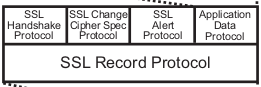
\includegraphics[width=0.25\textwidth]{img/tls-sub-protocols.png}
\caption{\label{fig:tls-subprotocols} TLS (Sub)protocols and Layers}
\end{wrapfigure}

Figure \ref{fig:tls-subprotocols} shows the subprotocols composing tls.

\subsubsection{\gls{tls} Record Processing}
A \gls{tls} record must go through some processing before it can tbe sent over the netwrok.
This processing involves the following steps (\codeword{4} for \gls{tls} 1.2 and \codeword{3} for \gls{tls} 1.3):

\begin{enumerate}
  \item \textbf{Fragmentation} - the \codeword{\gls{tls} Record Layer} takes arbitrary-length data and \textbf{fragments}
  it into manageable pieces: each one of the resulting fragments is called a \codeword{TLS Plaintext}.
  \item  \textbf{Compression} (removed in \gls{tls} 1.3) - the \codeword{TLS Record Layer} compresses the
  \codeword{TLSPlaintext} structure according to the negotiated compression method,
  outputting \codeword{TLSCompressed}. Compression is optional. If the negotiated compression
  method is \codeword{null}, \codeword{TLSCompressed} is the same as \codeword{TLSPlaintext}.
  \item \textbf{Cryptographic Protection} - in case of \gls{tls} 1.2, either an
  \gls{aead} cipher or a separate encryption and \gls{mac} functions transform a
  \codeword{TLSCompressed} fragment into a \codeword{TLSCipherText} fragment. In case
  of \gls{tls} 1.3, the \codeword{TLSPlaintext} fragment is transformed into a \codeword{TLSCipherText}
  by applying an \gls{aead} cipher.
  \item Append the \textbf{TLS Record Header} - encapsulate \codeword{TLSCipherText}
  in a \codeword{TLS Record}.
\end{enumerate}

\begin{wrapfigure}{r}{0.4\textwidth}
\centering
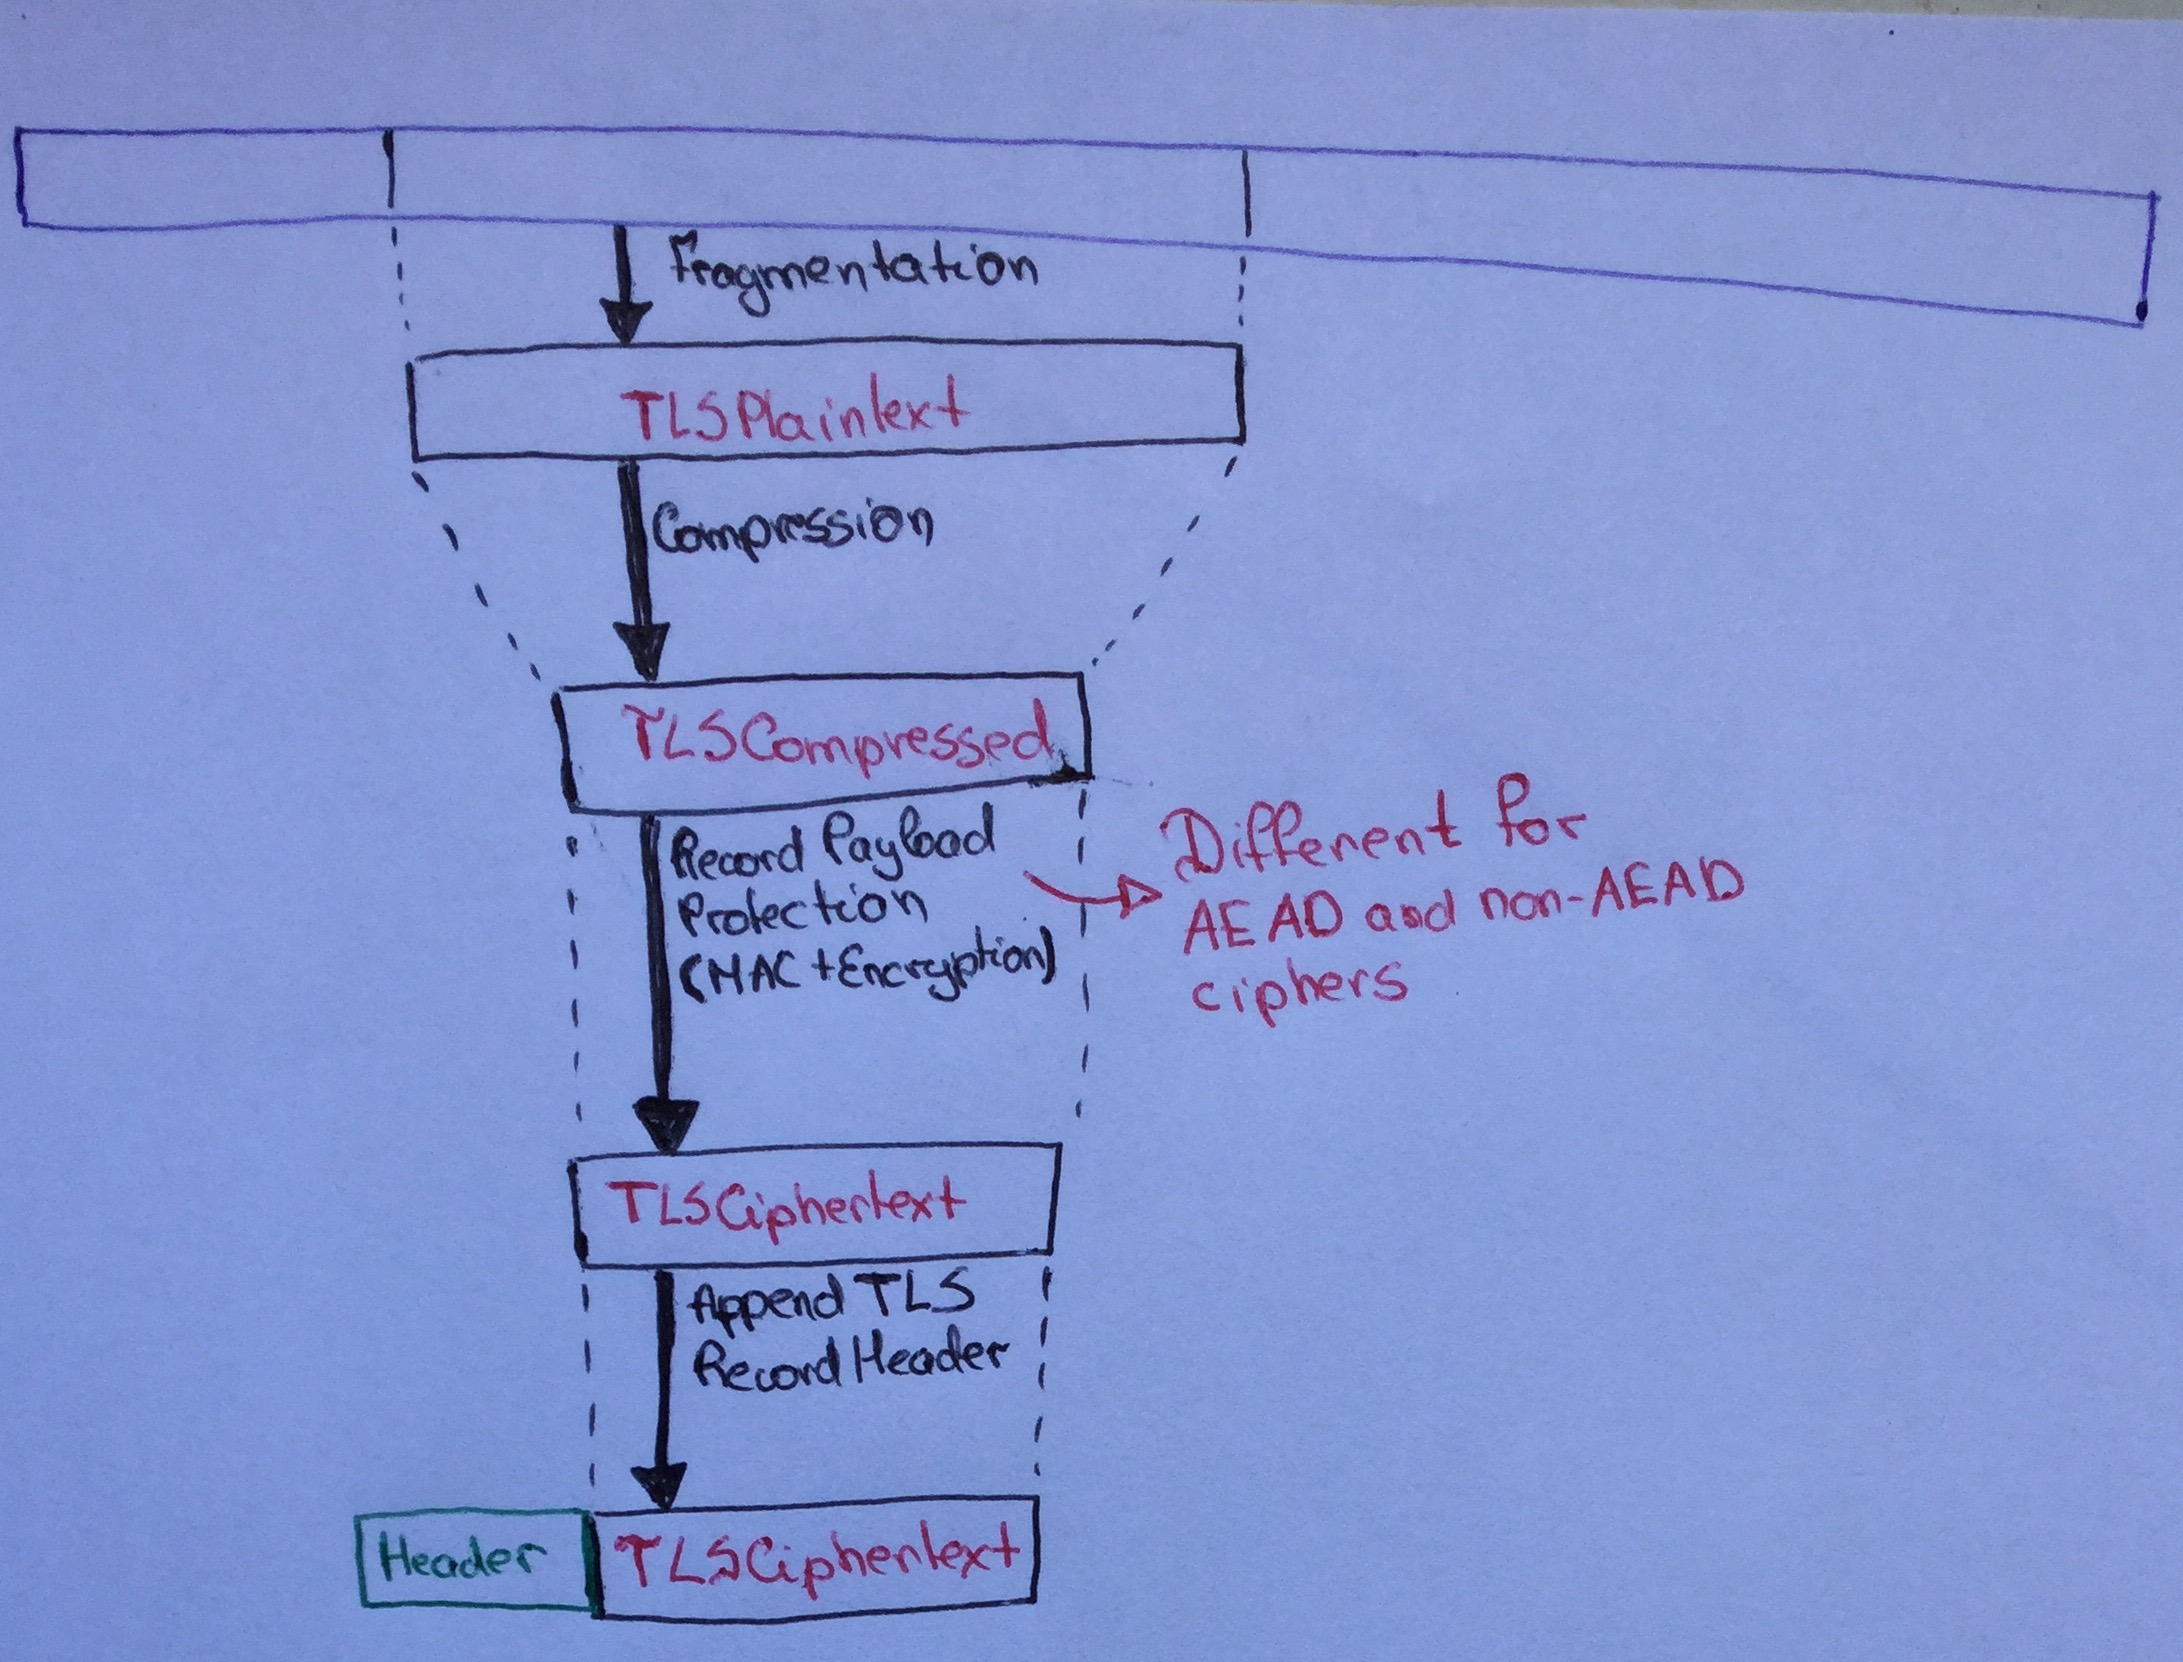
\includegraphics[width=0.7\textwidth]{img/tls-record-processing.jpg}
\caption{\label{fig:tls-record-processing}TLS Record Processing}
\end{wrapfigure}

The process described above, as well as the structure names are depicted in figure \ref{fig:tls-record-processing}.
Step \codeword{2} is not present in \gls{tls} 1.3. The structure names are exactly as the appear in the \gls{tls} specifications.

With this the common description of the \gls{tls} of protocols ends and we'll jump
into the specifics of the two verions. I'll be mostly concentrating on the
 \textbf{Handshake Protocol}, since this is where my work will be concentrated and
 it's the main part, where the most interesting and important things happen.

\subsection{TLS 1.2}
The latest standardized version of \gls{tls} is 1.2.

%
\paragraph{Notes and Comments.}
This is an example of a paragraph. Note the styling.

\subsection{TLS 1.3}
Despite the protocol name not suggesting it \gls{tls} 1.3 is
very different from \gls{tls} 1.2, in fact, it should've probably been called
\gls{tls} 2.0 instead.

\subsubsection{How Do Peers Distinguish Different TLS Versions?}

\todo{Talk about version numbers}

\subsection{TLS Extension Mechanism}

\todo{Describe the Extended ClientHello/ServerHello. Use one description for both,
 TLS 1.2 and TLS 1.3}

%
% ---- Bibliography ----
%
\nocite{*}
\bibliographystyle{splncs03}
\bibliography{tls_for_iot}
%
\printglossary[style=long]
%
\end{document}
